\documentclass[]{article}

\usepackage{caption,subcaption,graphicx,float,url,amsmath,amssymb,amsthm,tocloft,cancel}
\usepackage[toc,nonumberlist]{glossaries}
\usepackage{glossaries-extra,thmtools,gensymb,braket,bm,tensor}
\usepackage[toc,page]{appendix}

\newcommand\numberthis{\addtocounter{equation}{1}\tag{\theequation}}

\newtheorem{thm}{Theorem}
\newtheorem{defn}[thm]{Definition}
\newtheorem{cor}[thm]{Corollary}
\newtheorem{lemma}[thm]{Lemma}
\graphicspath{{figs/}}
\widowpenalty10000
\clubpenalty10000
\setcounter{tocdepth}{2}

%opening
\title{Theoretical Minimum\\General Relativity}
\author{}

\begin{document}

\maketitle

\begin{abstract}
	These are my notes for the \emph{General Rrlativity}\cite{susskind2012general} lectures from Leonard Susskind's \emph{Theoretical Minimum} series\cite{susskind2007theoretical}.
\end{abstract}

\tableofcontents
\listoffigures
\listoftables
\listoftheorems

\section{The Equivalence Principle \& Tensor Analysis}

LS begins where Einstein started. Einstein started with the simplest things and deduced far racing conclusions.

\subsection{The Equivalence Principle}

This is the principle that gravity is, in some sense, the same as acceleration.

\subsubsection{Coordinate Transformations}

If we are in an accelerated frame of reference, an elevator moving up or down say, we feel a gravitational field. Children know that.

Figure \ref{fig:gr-1-elevator} depicts an elevator. Assuming we know the laws of physics in the $z$ frame, surely we can figure then out in $z^\prime$.

\begin{figure}[H]
	\begin{center}
		\caption[Moving Elevator]{Moving Elevator: there are two coordinate systems, $z$ and $z^\prime$, and $L(t)$ allows us to pass from one to the other.}\label{fig:gr-1-elevator}
		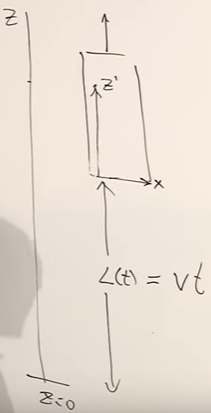
\includegraphics[width=0.4\textwidth]{gr-1-elevator}
	\end{center}
\end{figure}

In this lecture we'll ignore Special Relativity, which is tantamount to setting $c=\infty$ or assuming all velocities very small. If General Relativity is the generalization of Special Relativity, how did Einstein get away with ignoring Special Relativity? The answer is that Special Relativity is about high velocities. Gravity has to do with heavy masses. There are situation where the mass is high, but the velocity isn't. Einstein started thinking about these situations, and then combined it with Special Relativity to think about the combination of high masses and high velocities.

Let's think about inertial reference frames. If $z$ and $z^\prime$ are inertial, they are related by uniform velocity, so we have the coordinate transformation:

\begin{align*}
	L(t)=&vt\\
	z^\prime =& z-L(t)\\
	=& z-vt\\
	t^\prime =& t\\
	x^\prime =& x
\end{align*}

Now introduce Newton's 2nd law of motion. How does this change under the coordinate transformation?

\begin{align*}
	F =& m \ddot{z} \text{ in the $z$ frame}\\
	\ddot{z^\prime} =& \ddot{z} \text{ since $v$ is constant, whence:}\\
	F =& m \ddot{z^\prime} \text{ since $v$ is constant, so Newton's 2nd Law holds.}
\end{align*}

Now let's go to an accelerated frame--Figure \ref{fig:gr-1-elevator-accelerated}.

\begin{figure}[H]
	\begin{center}
		\caption{Elevator in a accelerated Frame}\label{fig:gr-1-elevator-accelerated}
		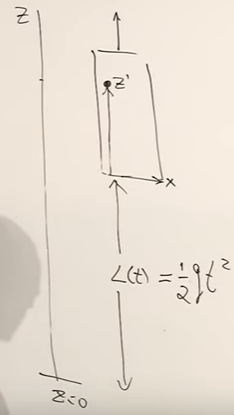
\includegraphics[width=0.4\textwidth]{gr-1-elevator-accelerated}
	\end{center}
\end{figure}

The coordinate transformation is now:
\begin{align*}
	L(t)=&vt\\
	z^\prime =& z-\frac{1}{2}g t^2\\
	=& z-vt\\
	t^\prime =& t\\
	x^\prime =& x
\end{align*}

We will continue to assume that Newton's laws hold in the $z$ frame of reference.
\begin{align*}
	\ddot{z^\prime} =& \ddot{z}-g\\
	\underbrace{F -mg}_\text{Force, including fictitious term} =& m \ddot{z^\prime} 
\end{align*}

The fictitious force looks like a uniform gravitational field. The special property of gravity is that gravitational forces are proportional to mass. That has a deep implication: the mass cancels, so the motion doesn't depend on the mass. Most people before Einstein considered this largely an accident. People know that acceleration mimicked gravity; Einstein said it was deep principle of nature. Figure \ref{fig:gr-1-coordinates-const} shows the coordinate transformation for constant velocity. Straight lines go to straight lines. Figure \ref{fig:gr-1-coordinates-accelerated} shows the results of accelerating the coordinate system: straight lines are not preserved. We have a curvy linear transformation. Einstein understood very early that there is a connection between gravity and curvy linear transformations of spacetime. Special Relativity was all about linear transformations

\begin{figure}[H]
	\begin{center}
		\caption{Coordinate Transformation for constant velocity versus accelerated}
		\begin{subfigure}[t]{0.45\textwidth}
			\caption{Coordinate Transformation for constant velocity. Green represents 	constant $z^\prime$}\label{fig:gr-1-coordinates-const}
			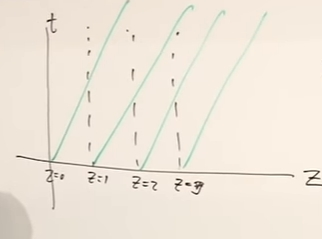
\includegraphics[width=\textwidth]{gr-1-coordinates-const}
		\end{subfigure}
		\;
		\begin{subfigure}[t]{0.4\textwidth}
			\caption{Coordinate Transformation 		accelerated}\label{fig:gr-1-coordinates-accelerated}
			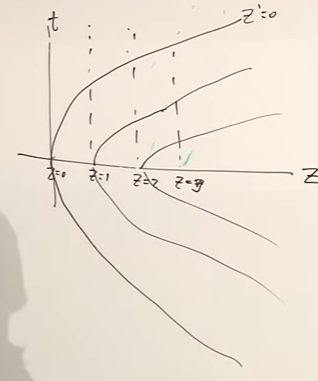
\includegraphics[width=\textwidth]{gr-1-coordinates-accelerated}
		\end{subfigure}
	\end{center}
\end{figure}



\subsubsection{Example: what is the influence of gravity on light?}
In 1907 most physicists would have thought there was no effect. Einstein argued from the equivalence principle that gravity would affect light. Consider a beam of light in our elevator--Figures \ref{fig:gr-1-light-in-elevator} and \ref{fig:gr-1-elevator-accelerated-curved-path}.

\begin{figure}[H]
	\caption{What is the influence of gravity on light? }
	\begin{subfigure}[t]{0.5\textwidth}
		\caption{Path of Light in $z$ system}\label{fig:gr-1-light-in-elevator}
		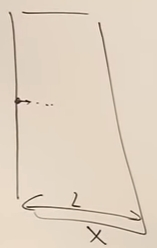
\includegraphics{gr-1-light-in-elevator}
	\end{subfigure}
	\begin{subfigure}[t]{0.5\textwidth}
		\caption{Path of Light in $z^\prime$ system}\label{fig:gr-1-elevator-accelerated-curved-path}
		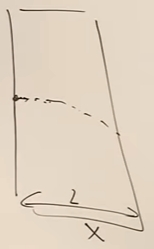
\includegraphics{gr-1-elevator-accelerated-curved-path}
	\end{subfigure}
\end{figure}

We'll write down the equation for the path of the light beam:
\begin{align*}
	x =& ct \text{ in the $z$ frame, and}\\
	z =& 0 \text{; in the moving frams}\\
	z^\prime + g\frac{t^2}{2} =&0 \text{, which is curved--Figure \ref{fig:gr-1-elevator-accelerated-curved-path}}
\end{align*}

\begin{itemize}
	\item In the primed system light is bending down;
	\item In the unprimed system the elevator is accelerating--the beam only \emph{looks} curved.
\end{itemize}

Einstein said that they are both the same thing.

What we have learned. 

\begin{enumerate}
	\item It is interesting to think about curvy linear transformations. 
	\item When you think about curvy linear transformations the form of Newton's Laws changes.
	\item One thing that happens is that apparent  gravitational fields  materialize that are apparently indistinguishable from ordinary gravitational fields.
\end{enumerate}

But are they really indistinguishable? Not really. Let's talk about gravitational fields generated by the Sun or the Earth--Figure \ref{fig:gr-1-suns-gravitational-field}. It is pretty obvious that there is no way to do a coordinate transformation like the ones we've been discussing which will remove the gravitational field. In \ref{fig:gr-1-suns-gravitational-field-local} we are in a laboratory we can transform away the field locally,  but there is no way to get rid of the fact that we are dealing with a field that is inwards globally.

\begin{figure}[H]
	\begin{center}
		\caption{Sun's Gravitational Field}
		\begin{subfigure}[t]{0.45\textwidth}
			\caption{There is no way to do a coordinate transformation like the ones we've 	been discussing which will remove the gravitational field}\label{fig:gr-1-suns-gravitational-field}
			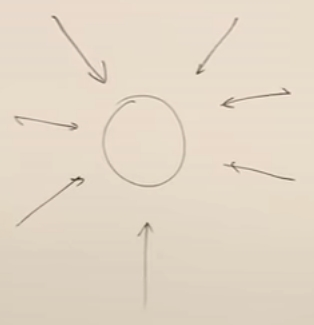
\includegraphics[width=\textwidth]{gr-1-suns-gravitational-field}
		\end{subfigure}
		\;
		\begin{subfigure}[t]{0.45\textwidth}
			\caption{If we are in a laboratory we can transform away the field locally, but 	there is no way to get rid of the fact that we are dealing with a field that is inwards globally.}\label{fig:gr-1-suns-gravitational-field-local}
			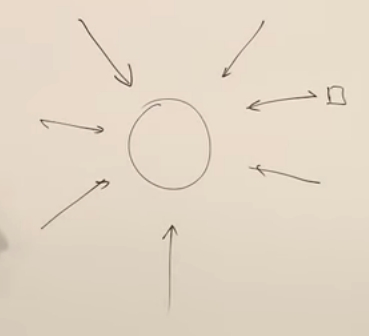
\includegraphics[width=\textwidth]{gr-1-suns-gravitational-field-local}
		\end{subfigure}
	\end{center}
\end{figure}

Figure \ref{fig:2000:mile:man} shows why we can't transform the field away. In Figure \ref{fig:gr-1-suns-gravitational-field-2000-mile-ff} 2000 Mile Man is oriented with his feet towards the Sun: he feels a tidal pull, as his feet are closer to the Sun than his head. In Figure \ref{fig:gr-1-suns-gravitational-field-2000-mile} he feels pressure at his head and feet. Being squashed is not something we can get rid of by performing a coordinate transformation. So it is not true that gravity is equivalent to a coordinate transformation. Einstein said that for small objects and small times, gravity was equivalent to a coordinate transformation.
\begin{figure}[H]
	\begin{center}
		\caption{The adventures of 2000 mile man}\label{fig:2000:mile:man}
		\begin{subfigure}[t]{0.45\textwidth}
			\caption{ 2000 Mile Man is oriented with his feet towards the Sun: he feels a 	tidal pull, as his feet are closer to the Sun than his head. }\label{fig:gr-1-suns-gravitational-field-2000-mile-ff}
			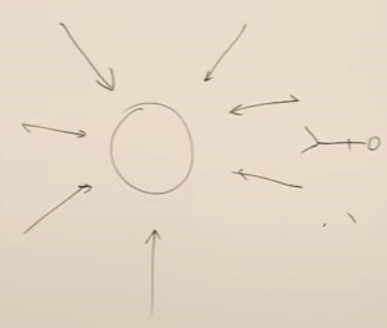
\includegraphics[width=\textwidth]{gr-1-suns-gravitational-field-2000-mile-ff}
		\end{subfigure}
		\;
		\begin{subfigure}[t]{0.45\textwidth}
			\caption{This time our hero feels pressure at his head and feet. Being squashed 	is not something we can get rid of by performing a coordinate transformation.}\label{fig:gr-1-suns-gravitational-field-2000-mile}
			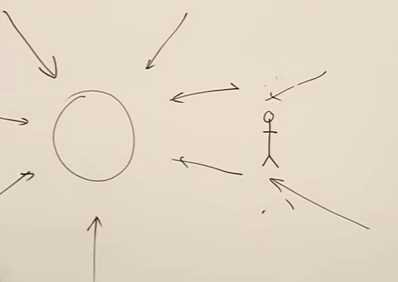
\includegraphics[width=\textwidth]{gr-1-suns-gravitational-field-2000-mile}
		\end{subfigure}
	\end{center}
\end{figure}

That raises a question: if I present you with a force field, e.g. the force field of uniform acceleration--Figure \ref{fig:gr-1-uniform-force-field}--you can make it look more complicated via a suitable transformation. If a transformation involve the $x$ axis it can make the field bend, or accelerate along $z$ while oscillating along $x$. This will give a complicated apparent gravitational field. If I tell you what the field is everywhere, how do I determine if it is just a fake gravitational field, from acceleration, or a real genuine one? If it is Newtonian gravitational field, just calculate the tidal forces on a freely falling object. If there is squeezing or stretching we have gravity,  otherwise not. If you can transform the field away it is not real gravity, otherwise it is real (can detect tidal forces via crystal).

\begin{figure}[H]
	\begin{center}
		\caption{Uniform Force Field}\label{fig:gr-1-uniform-force-field}
		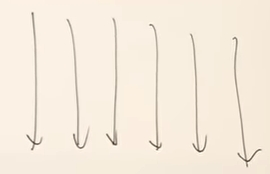
\includegraphics[width=0.5\textwidth]{gr-1-uniform-force-field}
	\end{center}
\end{figure}


Einstein asked what kind of mathematics he needed to answer the questions about real and apparent gravitational fields. The other element was special relativity: he know from the work of Minkowski that special relativity had a geometry associated with it, which had a length, proper distance.

\begin{align*}
	d\tau^2 =& dt^2 - dx^2 \text{, or, depending on who you are}\\
	ds^2 =& dx^2 -dt^2
\end{align*}

Einstein realized that the problem of deciding whether or not a gravitation field was real was similar to a problem that Riemann had explored, deciding whether or not a space was flat. Riemann had not considered metrics with a minus sign. In Euclidean space:
\begin{align*}
	ds^2 =& \sum (dx^i)^2 \numberthis \label{eq:euclidean:metric}
\end{align*}
 
Gauss had already understood that in non-Euclidean spaces the formula for distance on a surface was more complicated. Riemann took the next step. Consider a curved surface (let's not worry what this means exactly), and lay out coordinates as in Figure \ref{fig:gr-1-curved-surface-coordinates}.
 
\begin{figure}[H]
	\begin{center}
		\caption[Curved Surface with coordinates]{Curved Surface with coordinates. Don't worry about straight lines.}\label{fig:gr-1-curved-surface-coordinates}
		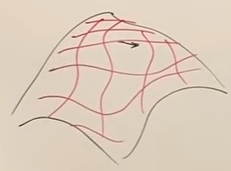
\includegraphics{gr-1-curved-surface-coordinates}
	\end{center}
\end{figure} 

The formula for the distance between two close points becomes:
\begin{align*}
	ds^2 =& \sum_{m,n} g_{mn}(x) dx^m dx^n
\end{align*}
It works also for curved coordinates in a flat space.

We are building up geometry in little regions and piecing them together. Maybe we can put them together on a flat plane, but maybe not. So, given the little pieces, how do we know whether or not it is flat? Is there a coordinate system where (\ref{eq:euclidean:metric}) holds?

We have two parallel questions. Can we find a coordinate system:
\begin{itemize}
	\item where apparent gravitational field is zero;
	\item where (\ref{eq:euclidean:metric}) is true.
\end{itemize}

We will need the mathematics of Tensor Analysis.

\subsection{Tensor Analysis}

Can we change $g_{mn}$ to $\delta_{mn}$? First question is how does $g_{mn}$ change when we change coordinates?

We have two sets of coordinates, $x$ and $y$, and write $x^m = x^m(y)$, and $y^m = y^m(x)$. How do $dx_m$ transform?

\begin{align*}
	dy^m =& \sum_p \frac{\partial y^m}{\partial x^p} dx^p\\
	V^{\prime m} =& \sum_p \frac{\partial y^m}{\partial x^p} V^p \text{, or, using Einstein's summation convention} \\
	V^{\prime m} =&  \frac{\partial y^m}{\partial x^p} V^p \numberthis \label{eq:contravariant}
\end{align*}

\begin{defn}[Contravariant]
	A Vector whose components transform in accordance with (\ref{eq:contravariant}) is said to be \emph{contravariant}.
\end{defn}

Consider a scalar function, $s$, then the gradient is a vector.

\begin{defn}[Gradient]
	The gradient of $s$ is $\frac{\partial s}{\partial x^p}$.
\end{defn}

\begin{align*}
	\frac{\partial s}{\partial y^m} =& \frac{\partial s}{\partial x^p}\frac{\partial x^p}{\partial y^m}\\
	W_m^\prime =& \frac{\partial x^p}{\partial y^m} W_p \numberthis \label{eq:covariant}
\end{align*}

\begin{defn}[Covariant]
	A Vector whose components transform in accordance with (\ref{eq:covariant}) is said to be \emph{covariant}.
\end{defn}
 
Relativity is about the transformation properties of objects.

To define more general tensors, consider products of vectors -- e.g.
\begin{align*}
	V^mU^n=&T^{mn} \text{, contravariant tensor of rank 2 }
\end{align*}

LS derived the transformation properties, and showed that $g_{mn}$ is covariant.


\section{Tensor mathematics}

A good notation will carry you a long way. When it is good it tells you what to do next. It's like tinker toys: you put the stick into a hole. The notation of GR is like that: if you follow the rules it is difficult to make mistakes. The rules are tensor analysis and tensor algebra.

\subsection{Flat space}

Our aim is to distinguish flat from not flat. LS rolls flat page into cylinder, which is locally flat (it has extrinsic curvature from the embedding in 3D, not intrinsic: a tiny bug embedded in the surface can't notice this sort of curvature, but can find intrinsic curvature). Riemannian geometry is about intrinsic properties of space.
 
Figures \ref{fig:gr-2-lattice} and \ref{fig:gr-2-lattice-not-flat} illustrate a surface can be flattened and one that cannot. A curved surface is one that cannot be flattened without distorting it.

\begin{figure}[H]
	\caption{Can we flatten the lattice onto a surface?}
	\begin{subfigure}[t]{0.5\textwidth}
		\caption{Flat Lattice of equilateral triangles. These can be drawn on a plane.}\label{fig:gr-2-lattice}
		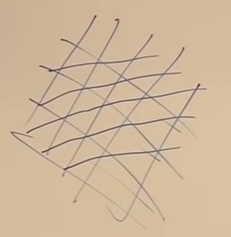
\includegraphics[width=\textwidth]{gr-2-lattice}
	\end{subfigure}
	\begin{subfigure}[t]{0.5\textwidth}
		\caption{Not a Flat Lattice: the bold lines are twice the length of the others, so the central one is forced up, out of blackboard.}\label{fig:gr-2-lattice-not-flat}
		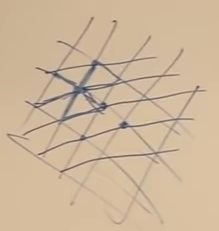
\includegraphics[width=\textwidth]{gr-2-lattice-not-flat}
	\end{subfigure}
\end{figure}

Our problem is to decide whether or not a space is really flat. What are we given? We are given a metric tensor.

\subsection{Transformations}

\subsubsection{Scalars transform trivially}

\begin{align*}
	x^m \leftrightarrow& y^m \\
	S^\prime(y) =& S(x) \text{, we call such an $s$ a scalar}
\end{align*}

\subsubsection{Contravariant \& Covariant Vectors}

Figure \ref{fig:gr-2-coordinates} depicts a coordinate system, and a vector $\vec{V}$.
\begin{figure}[H]
	\caption[A set of coordinates, not necessarily perpendicular.]{A set of coordinates, not necessarily perpendicular (although they could be). Furthermore the distances along the axes are just labels: they need not be equidistant. There are two unit vectors, $\vec{e_1}$ and $\vec{e_2}$ along the $x_1$ and $x_2$ axes.}\label{fig:gr-2-coordinates}
	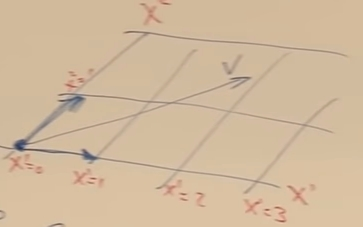
\includegraphics{gr-2-coordinates}
\end{figure}

$\vec{V}$ can be expanded:
\begin{align*}
	\vec{V} =& \sum_i V^i \vec{e_i} \numberthis \label{eq:contravariant:components}
\end{align*}

\begin{defn}[Contravariant components]
	 In (\ref{eq:contravariant:components}), the numbers $V_i$ are called the\emph{ contravariant components} of $\vec{V}$.
\end{defn}

What is $\vec{V} \boldsymbol{\cdot} \vec{e_1}$? If the coordinate system were rectangular, and the labels were equally spaced, it would be $V^1$. As things stand we define:
\begin{align*}
	V_n \triangleq & \vec{V} \boldsymbol{\cdot} \vec{e_n} \numberthis \label{eq:covariant:components}\\
	=& V^m \underbrace{\vec{e_m}\boldsymbol{\cdot} \vec{e_n}}_\text{The metric tensor $g_{mn}$} \numberthis \label{eq:metric_tensor}
\end{align*}

\begin{defn}[Covariant components]
	In (\ref{eq:covariant:components}), the numbers $V^i$ are called the\emph{ covariant components} of $\vec{V}$.
\end{defn}

Let's compute the length of $\vec{V}$.

\begin{align*}
	\vec{V}\boldsymbol{\cdot} \vec{V} =& V^m \vec{e_m}\boldsymbol{\cdot} V^n \vec{e_n}\\
	=& V^m V^n (\vec{e_m}\boldsymbol{\cdot} \vec{e_n})\\
	=&  V^m V^n g_{mn} \text{, where we define $g_{m,n}$ as in (\ref{eq:metric_tensor})}
\end{align*}

If the coordinates are perpendicular, and the separations are the same, the distinction between covariant and contravariant disappears. Polar coordinates are orthogonal, but the separations are not the same.

NB: covariant and contravariant vectors are two different things. Once you introduce a metric tensor it is possible to transform one to the other.

\begin{align*}
	V^{\prime m} =&  \frac{\partial y^m}{\partial x^p} V^p \text{, contravariant transformation}\\
	\frac{\partial S}{\partial y^m} =& \frac{\partial x^p}{\partial y^m} \frac{\partial S}{\partial x^p} \text{, covariant transformation}\\
	W_m^\prime =& \frac{\partial x^p}{\partial y^m} W_p
\end{align*}

I've omitted a discussion of higher rank tensors, which is based on products.

Also if a tensor is zero in one frame it is zero in all frames: if a tensor equation is true in one frame it is true in all frames.

\subsection{Tensor mathematics: addition, multiplication, contraction}

\begin{enumerate}
	\item Addition
	\item Multiplication of Tensors
	\item Contraction
	\item Covariant differentiation
\end{enumerate}

LS presents usual properties, and shows that $g_{mn}$ is a symmetric tensor. He points out that eigenvalues cannot be zero, as otherwise we'd have an elementary vector of zero length. Hence it has an inverse: $g^{mn}g_{np}=\delta_m^p$.


\section{Flatness \& curvature}

''General Relativity has a reputation for being very difficult. I think the reason is because it's very difficult.''--Leonard Susskind

\subsection{Flatness}

A flat geometry is one where all Euclid's postulates are true. It is characterized in terms of the metric: not that $g_{i,j} = \delta_{i,j}$, but rather that coordinates can be found where the metric has such a simple form. More generally, given a metric that is smooth and has all the good differentiable properties, the problem of determining whether or not that space is flat is somewhat difficult. The bad way is to consider all coordinate systems, calculate the metric, and calculate whether it has the required form. The good way is to look for diagnostic quantities, things you can calculate which, if they are zero everywhere the space is flat; if they are non-zero anywhere it means the space is curved there. The diagnostic quantity is called the curvature tensor.

Where want to find a tensor $R$ such that $R=0$ in a flat space.

\begin{align*}
	ds^2 =& g\indices{_{mn}}(x) dx^m dx^n\\
	\exists  g\indices{^{mn}} \mid  g\indices{^{mn}} g\indices{_{nr}} =& \delta\indices{^m_r}\\
	V^m g_{mn} =& V_n\\
	V_m g^{mn} =& V^n
\end{align*}
 
 In Riemannian geometry, unlike Einsteinian, $ds^2 \ge 0$.
 
 \begin{thm}[Gaussian Normal coordinates--Figure \ref{fig:gr-4-gaussian-normal}]
 	At every point, $x_0$ you can choose coordinates such that:
 	\begin{align*}
 	g_{mn}(x_0)=&\delta_{mn}, \text{, and} \numberthis \label{eq:gnf1}\\
 	\frac{\partial g_{m,n}(x_0)}{\partial x^r}=&0 \numberthis \label{eq:gnf2}
 	\end{align*}
 \end{thm}

\begin{figure}[H]
	\begin{center}
		\caption{Gaussian Normal Form}\label{fig:gr-4-gaussian-normal}
		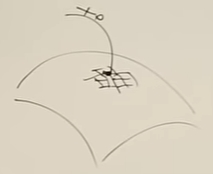
\includegraphics{gr-4-gaussian-normal}
	\end{center}
\end{figure}

\begin{proof}
	Start with some coordinates $y$ and derive new coordinates $x$.
	\begin{align*}
		x^m = y^m + c\indices{^m_{nr}} y^n y^r \text{, assume the same origin.}
	\end{align*}
	In 4 dimensional space there are 40 combinations of $m$, $n$ and $r$; there are 40 coefficients $c\indices{^m_{nr}}$. Moreover (\ref{eq:gnf2}) is actually 40 equations, so we can choose the $c\indices{^m_{nr}}$ so (\ref{eq:gnf2})  is satisfied.
	How do we get the flat metric?
\end{proof}
The problem is that we can't extend away from $x_0$, except in a flat space. The problem is the second derivatives. In general $\frac{\partial^2 g_{m,n}(x_0)}{\partial x^r \partial x^s}\ne0$. The metric is locally flat.

\subsection{Gaussian normal coordinates}

\begin{itemize}
	\item Can we construct a derivative of a tensor?
	\item What does it mean for one vector to be the same as another at a different point? Equality of components isn't enough--Figure \ref{fig:gr-4-equality-of-vectors}. 
\end{itemize}

\begin{figure}[H]
	\begin{center}
		\caption[What does it mean for one vector to be the same as another at a different point?]{What does it mean for one vector to be the same as another at a different point? $\frac{\partial V_m}{\partial V^n}=0$ is not a tensor equation, therefore $\frac{\partial V_m}{\partial V^n}$ is not a tensor.}\label{fig:gr-4-equality-of-vectors}
		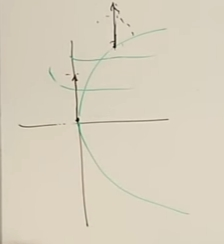
\includegraphics{gr-4-equality-of-vectors}
	\end{center}
\end{figure}

\subsection{Covariant Derivatives}

We need a better definition of the derivative of a vector.

\begin{enumerate}
	\item Create Gaussian normal coordinates.
	\item Pretending that the Gaussian normal coordinates are nice flat coordinates, shift the second vector so its origin is the same as the original vector and the coordinates--Figure \ref{fig:gr-4-equality-of-vectors-revised}.
	\item Take the difference between the two vectors.
	\item Our difference takes into account the change in the vector, and the change in the coordinate system.
\end{enumerate}

\begin{figure}[H]
	\begin{center}
		\caption{Shift the second vector so its origin is the same as the original}\label{fig:gr-4-equality-of-vectors-revised}
		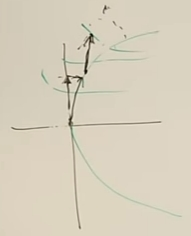
\includegraphics{gr-4-equality-of-vectors-revised}
	\end{center}
\end{figure}

We find:
\begin{align*}
	D_r V_m =& \partial r V_{m} - \Gamma\indices{^t_{rm}} V^t \text{, covariant derivative.} \numberthis \label{eq:covariant_1}\\
	\Gamma\indices{^t_{rm}} =& \Gamma\indices{^t_{rm}}\numberthis \label{eq:symmetry:Gamma}\\
	D_r T_{mn} =& \partial_r T_{mn} - \Gamma\indices{^t_{rm}} T_{tn} - \Gamma\indices{^t_{rn}} T_{mt} \numberthis \label{eq:covariant_2}
\end{align*}

$\Gamma$ is known a "connection", or a Christoffel symbol; which contains various $\frac{\partial g_{m,n}}{\partial x^r}$, which are zero in Gaussian Normal coordinates.

\begin{lemma}[$D_r g_{mn}=0$]\label{thm:covariant_derivative:metric}
	The covariant derivative of the metric tensor is zero.
\end{lemma}

\begin{proof}
	The result follows from the fact that the metric tensor has zero derivatives at $x_0$ in Gaussian Normal coordinates, and the definition of covariant derivative is to differentiate in Gaussian Normal coordinates and treat the result as a tensor.
\end{proof}

\begin{thm}[Christoffel symbols]
	\begin{align*}
		\Gamma\indices{^t_{mn}} =& \frac{1}{2}\big[\partial_n g_{sm} + \partial_m g_{sn}- \partial_s g_{mn}\big]  g^{st}   \numberthis \label{eq:christoffel}
	\end{align*}
\end{thm}

\begin{proof}
	\begin{align*}
		D_s g_{mn} =& \partial_s g_{mn} - \Gamma\indices{^t_{sm}} g_{tn} - \Gamma\indices{^t_{sn}} g_{tm} 	=& 0 \numberthis \label{eq:D:d:1}\\
		D_m g_{sn} =& \partial_m g_{sn} - \underbrace{\Gamma\indices{^t_{sm}}}_\text{From (\ref{eq:symmetry:Gamma})} g_{tn} - \Gamma\indices{^t_{mn}} g_{st} 	=& 0 \numberthis \label{eq:D:d:2}\\
		D_n g_{sm} =& \partial_n g_{sm} - \Gamma\indices{^t_{sn}} g_{tm} - \Gamma\indices{^t_{mn}} g_{st} 	=& 0 \numberthis \label{eq:D:d:3}
	\end{align*}
	
	Now we take (\ref{eq:D:d:3}) + (\ref{eq:D:d:2}) - (\ref{eq:D:d:1}).
	
	\begin{align*}
		\partial_n g_{sm} + \partial_m g_{sn}- \partial_s g_{mn} =& \bcancel{\Gamma\indices{^t_{sn}} g_{tm}} + \Gamma\indices{^t_{mn}} g_{st} + \cancel{\Gamma\indices{^t_{sm}}g_{tn}} + \Gamma\indices{^t_{mn}} g_{st} - \cancel{\Gamma\indices{^t_{sm}} g_{tn}} - \bcancel{\Gamma\indices{^t_{sn}} g_{tm}} \\
		=&2 \Gamma\indices{^t_{mn}} g_{st} \text{, whence}\\
		\Gamma\indices{^t_{mn}} =& \frac{1}{2}\big[\partial_n g_{sm} + \partial_m g_{sn}- \partial_s g_{mn}\big]  g^{st} \numberthis \label{eq:christoffel:g}  
	\end{align*}
\end{proof}

\subsection{The Riemann Curvature Tensor}

We want to define curvature. Consider Figures \ref{fig:gr-4-curved-cone} and \ref{fig:gr-4-curved-cone-vector-field} show that the direction of a vector field changes if we transport it around in a surface that is curved, even though we transported it parallel to itself, i.e. the covariant derivative was zero.
\begin{figure}[H]
	\begin{center}
		\caption{Illustrating curvature}
		\begin{subfigure}[t]{0.4\textwidth}
			\caption{A cone, which is flat everywhere except at the top.}\label{fig:gr-4-curved-cone}
			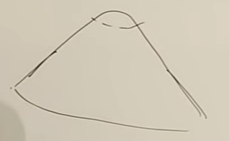
\includegraphics[width=0.9\textwidth]{gr-4-curved-cone}
		\end{subfigure}
		\;
		\begin{subfigure}[t]{0.4\textwidth}
			\caption{Vector field is transported around cone: angle to cut changes!}\label{fig:gr-4-curved-cone-vector-field}
			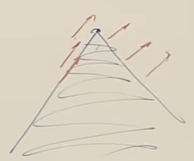
\includegraphics[width=0.9\textwidth]{gr-4-curved-cone-vector-field}
		\end{subfigure}
	\end{center}
\end{figure}

Figure \ref{fig:gr-4-2D} transports a vector along two paths. In a flat space two transported vectors will be identical, $D_r D_s V_m = D_s D_r V_m$, but this is not true in curved space.
\begin{figure}[H]
	\begin{center}
		\caption{Compare vector along two paths}\label{fig:gr-4-2D}
		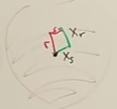
\includegraphics{gr-4-2D}
	\end{center}
\end{figure}

\begin{thm}[Riemann curvature tensor]
	\begin{align*}
		D_s D_r V_m - D_r D_s V_m =& R\indices{_{sr}^t_m} V_t \text{, where the Riemann curvature tensor is}\\
		R\indices{_{sr}^t_m} \triangleq & \partial_r \Gamma \indices{^t_{sm}} - \partial_s \Gamma \indices{^t_{rm}} + \Gamma \indices{^p_{sm}} \Gamma \indices{^t_{pr}}- \Gamma \indices{^p_{rm}} \Gamma \indices{^t_{ps}} 
	\end{align*}
\end{thm}

\begin{proof}
	\begin{align*}
		D_s D_r V_m =& D_s T_{rm} \text{, where}\\
		T_{rm}=& \partial_r V_m -\Gamma \indices{^t_{rm}} V_t \text{, whence}\\
		D_s D_r V_m	=& \partial_s T_{rm} - \Gamma\indices{^t_{sr}} T_{tm} - \Gamma\indices{^t_{sm}} T_{rt} \text{, from (\ref{eq:covariant_2})}\\
		=& \partial_s \big(\partial_r V_m -\Gamma \indices{^t_{rm}} V_t\big) - \Gamma\indices{^t_{sr}} \big(\partial_t V_m -\Gamma \indices{^u_{tm}} V_u\big) - \Gamma\indices{^t_{sm}} \big(\partial_r V_t -\Gamma \indices{^u_{rt}} V_u\big)\\
		=& \partial_s \partial_r V_m - \partial_s \big( \Gamma \indices{^t_{rm}} V_t\big) - \Gamma\indices{^t_{sr}}\partial_t V_m + \Gamma\indices{^t_{sr}} \Gamma \indices{^u_{tm}} V_u - \Gamma\indices{^t_{sm}} \partial_r V_t + \Gamma\indices{^t_{sm}}\Gamma \indices{^u_{rt}} V_u\\
		=& \partial_s \partial_r V_m - \partial_s \big( \Gamma \indices{^t_{rm}} \big)V_t -  \Gamma \indices{^t_{rm}}  \partial_s V_t - \Gamma\indices{^t_{sr}}\partial_t V_m +  \Gamma\indices{^t_{sr}} \Gamma \indices{^u_{tm}} V_u - \Gamma\indices{^t_{sm}} \partial_r V_t + \Gamma\indices{^t_{sm}}\Gamma \indices{^u_{rt}} V_u
	\end{align*}
	
	We interchange the subscripts $r$ and $s$ in the last equation, and then mark the terms that can be cancelled when we subtract, taking into account the symmetry of $g_{rs}$ and $\Gamma\indices{^._{rs}}$.
	
	\begin{align*}
		D_s D_r V_m =&\underbrace{\partial_s \partial_r V_m}_\text{I} - \partial_s \big( \Gamma \indices{^t_{rm}} \big)V_t -  \underbrace{\Gamma \indices{^t_{rm}}  \partial_s V_t}_\text{II} - \underbrace{\Gamma\indices{^t_{sr}}\partial_t V_m}_\text{IV} +  \underbrace{\Gamma\indices{^t_{sr}} \Gamma \indices{^u_{tm}} V_u}_\text{V} - \underbrace{\Gamma\indices{^t_{sm}} \partial_r V_t}_\text{III} + \Gamma\indices{^t_{sm}}\Gamma \indices{^u_{rt}} V_u\\
		D_r D_s V_m =&\underbrace{\partial_r \partial_r V_m}_I - \partial_r \big( \Gamma \indices{^t_{sm}} \big)V_t -  \underbrace{\Gamma \indices{^t_{sm}}  \partial_r V_t}_\text{III} - \underbrace{\Gamma\indices{^t_{rs}}\partial_t V_m}_\text{IV} +  \underbrace{\Gamma\indices{^t_{rs}} \Gamma \indices{^u_{tm}} V_u}_\text{V} - \underbrace{\Gamma\indices{^t_{rm}} \partial_s V_t}_\text{II} + \Gamma\indices{^t_{rm}}\Gamma \indices{^u_{st}} V_u
	\end{align*}
	
	Subtracting, and replacing summation indices in the last two terms, we have:
	\begin{align*}
		D_s D_r V_m - D_r D_s V_m =& \partial_r \big( \Gamma \indices{^t_{sm}} \big)V_t - \partial_s \big( \Gamma \indices{^t_{rm}} \big)V_t + \Gamma\indices{^t_{sm}}\Gamma \indices{^u_{rt}} V_u - \Gamma\indices{^t_{rm}}\Gamma \indices{^u_{st}} V_u\\
		=& \partial_r \big( \Gamma \indices{^t_{sm}} \big)V_t - \partial_s \big( \Gamma \indices{^t_{rm}} \big)V_t + \Gamma\indices{^p_{sm}}\Gamma \indices{^t_{rp}} V_t - \Gamma\indices{^p_{rm}}\Gamma \indices{^t_{sp}} V_t\\
		=& \big[\partial_r  \Gamma \indices{^t_{sm}}  - \partial_s \Gamma \indices{^t_{rm}} + \Gamma\indices{^p_{sm}}\Gamma \indices{^t_{rp}}  - \Gamma\indices{^p_{rm}}\Gamma \indices{^t_{sp}} \big] V_t
	\end{align*}
\end{proof}

The curvature tensor indicates whether or not a space is flat, and it includes the tidal forces.

In Figure \ref{fig:gr-3-move-links} we see the geometric interpretation of {$D_s D_r V_m - D_r D_s V_m$. It measures the stretching that happens when we move the structure of links into the curved region.

\begin{figure}[H]
	\caption[Geometric meaning of $D_s D_r V_m - D_r D_s V_m$]{$D_s D_r V_m - D_r D_s V_m$ measuring the stretching that happens when we move the structure of links into the curved region.}\label{fig:gr-3-move-links}
	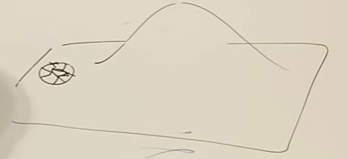
\includegraphics{gr-3-move-links}
\end{figure}


\section{Geodesics \& gravity}

\subsection{Review}

The point of a covariant derivative is to write a tensor such that in Gaussian Normal Coordinates it is just the derivative.

\begin{thm}[Covariant Derivative of contravariant vector]
	\begin{align*}
		D_m V^n =& \partial m V_n + \Gamma\indices{^n_{mr}} V^r
	\end{align*}
\end{thm}

\begin{proof}
	\begin{align*}
		D_m V^n =& D_m\big( g^{np} V_p\big)\\
		=&  \cancel{\big(D_m g^{np}\big) V_p} +  g^{np} D_m V_p \text{,  where we have used Lemma \ref{thm:covariant_derivative:metric}}\\
		=& g^{np} \big(\partial_m V_p -  \Gamma\indices{^r_{pm}} V_r\big) \text{, from (\ref{eq:covariant_1})}\\
		=& g^{np} \big[\partial_m \big(g_{pq} V^q\big) -  \Gamma\indices{^r_{pm}} g_{rq} V^q\big]\\
		=& g^{np} \big[ \partial_m \big(g_{pq} \big)V^q + g_{pq} \partial_m V^q -  \Gamma\indices{^r_{pm}} g_{rq} V^q\big]\\
		=& \cancel{g^{np} g_{pq}} \partial_m V^q +  g^{np} \big[ \partial_m \big(g_{pq} \big) -   \Gamma\indices{^r_{pm}} g_{rq} \big] V^q \numberthis\label{eq:cov:contra}
	\end{align*}
	Now, using (\ref{eq:christoffel:g})
	\begin{align*}
		 \partial_m g_{pq} -   \Gamma\indices{^r_{pm}} g_{rq} =&\partial_m \big(g_{pq} \big) - \frac{1}{2}\big[\partial_m g_{sp} + \partial_p g_{sm}- \partial_s g_{pm}\big]  \cancel{g^{sr} g_{rq}}\\
		=& \partial_m \big(g_{pq} \big) - \frac{1}{2}\big[\partial_m g_{sp} + \partial_p g_{sm}- \partial_s g_{pm}\big] \partial_m g_{pq} +   \Gamma\indices{^r_{pm}} g_{rq}\\
		 =& \frac{1}{2}\big[\partial_m g_{qp} - \partial_p g_{qm}+ \partial_q g_{pm}\big] 
	\end{align*}
	
	Using (\ref{eq:christoffel:g}) again:
	\begin{align*}
		g^{np} \big[ \partial_m \big(g_{pq} \big) -   \Gamma\indices{^r_{pm}} g_{rq} \big] V^q =& g^{np} \frac{1}{2}\big[\partial_m g_{qp} - \partial_p g_{qm}+ \partial_q g_{pm}\big] V^q\\
		=& \Gamma \indices{^n_{qm}} V^q \text{, and (\ref{eq:cov:contra}) becomes}\\
		D_m V^n =& \partial_m V^n +  \Gamma \indices{^n_{qm}} V^q
	\end{align*}
	
\end{proof}

\subsection{Parallel Transport}

Given a vector field, move along curve. Does vector remain parallel to itself, i.e. $D_m V^n=0$--Figure \ref{fig:gr-4-DV-along-curve}?

\begin{figure}[H]
	\caption{Parallel Transport}
	\begin{center}
		\begin{subfigure}[t]{0.3\textwidth}
			\caption{Transporting vector along curve}\label{fig:gr-4-DV-along-curve}
			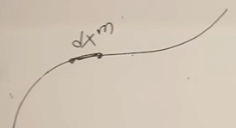
\includegraphics[width=\textwidth]{gr-4-DV-along-curve}
		\end{subfigure}
		\;
		\begin{subfigure}[t]{0.3\textwidth}
			\caption{Parallel Transport is path dependent}\label{fig:gr-4-parallel-transport-path-dependent}
			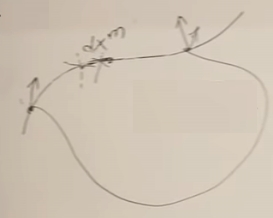
\includegraphics[width=\textwidth]{gr-4-parallel-transport-path-dependent}
		\end{subfigure}
		\;
		\begin{subfigure}[t]{0.3\textwidth}
			\caption{Transporting vectors around a cone gives different results, e.g. the bold portion of the curve versus the rest of the curve. }\label{fig:gr-4-cone-round}
			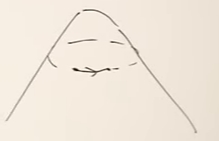
\includegraphics[width=\textwidth]{gr-4-cone-round}
		\end{subfigure}
	\end{center}
\end{figure}

\begin{align*}
	DV^n \triangleq& D_m V^v dx_m\\
	=& \underbrace{\frac{\partial V^n}{\partial x^m} dx^m}_\text{$\triangleq dV^n $} + \Gamma \indices{^n_{mr}} V^r dx^m
\end{align*}

\begin{defn}[Parallel transport]
	If $DV^n=0$ along the curve, we say it is being transported parallel to itself.
\end{defn}

\begin{thm}[Parallel transport preserved length]
	If $DV^n=0$ along the curve, the lenghth of V is preserved.
\end{thm}

\begin{proof}
	TBP
\end{proof}

The result of parallel transporting vector in curved space depends on the path--Figures \ref{fig:gr-4-parallel-transport-path-dependent} and \ref{fig:gr-4-cone-round}. 

\begin{figure}[H]
	\begin{center}
		\caption{In general the tangent vector to a curve is not covariantly constant}
		\begin{subfigure}[t]{0.3\textwidth}
			\caption{The cone modified with a sharp point, se we can unroll}\label{fig:gr-4-cone}
			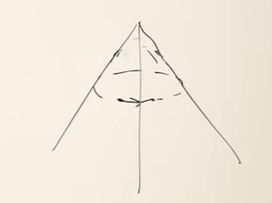
\includegraphics[width=\textwidth]{gr-4-cone}
		\end{subfigure}
		\;
		\begin{subfigure}[t]{0.3\textwidth}
			\caption{Open up the cone and transport a tangent vector, which is changed when it comes back to the original point. The two dots represent the same point.}\label{fig:gr-4-cone-sliced-tangent}
			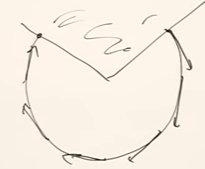
\includegraphics[width=\textwidth]{gr-4-cone-sliced-tangent}
		\end{subfigure}
		\;
		\begin{subfigure}[t]{0.3\textwidth}
			\caption{Add a second vector which maintains the same heading}\label{fig:gr-4-cone-sliced}
			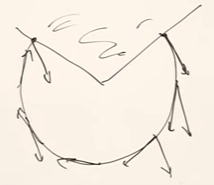
\includegraphics[width=\textwidth]{gr-4-cone-sliced}
		\end{subfigure}
	\end{center}
\end{figure}

 
Figures \ref{fig:gr-4-cone}, \ref{fig:gr-4-cone-sliced-tangent}, and \ref{fig:gr-4-cone-sliced} we slice the cone and open it up. This illustrates the fact that the tangent isn't always parallel to the curve; when it is, the curve is a geodesic, but the curve in Figure \ref{fig:gr-4-cone} is clearly not a geodesic.

\subsection{Geodesics} 

\begin{itemize}
	\item 	A geodesic is a curve whose distance it stationary.
	\item A better definition is to look locally along the curve and require that the curve be as straight as possible.
\end{itemize}

If along the curve the derivative of the tangent vector is zero, that curve is as straight as possible.

In Figure \ref{fig:gr-4-geodesic-intuition} we have a terrain with hills and valleys. We drive a car which is small compared to any curves in the terrain. Point steering wheel to dead straight and start driving without deviating: your path--Figure \ref{fig:gr-4-geodesic-intuition-path}--will be a geodesic.
\begin{figure}[H]
	\begin{center}
		\caption{Intuition for geodesics}
		\begin{subfigure}{0.45\textwidth}
			\caption{Terrain}\label{fig:gr-4-geodesic-intuition}
			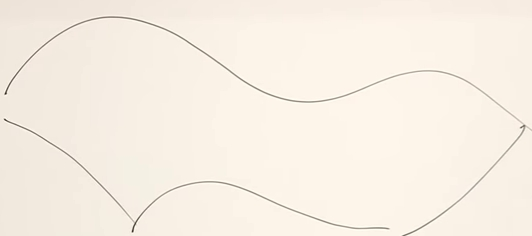
\includegraphics[width=\textwidth]{gr-4-geodesic-intuition}
		\end{subfigure}
		\begin{subfigure}{0.45\textwidth}
			\caption{Your path will be a geodesic}\label{fig:gr-4-geodesic-intuition-path}
			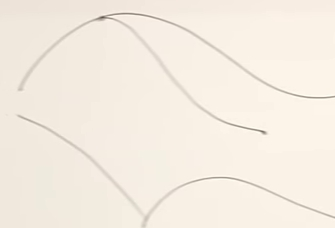
\includegraphics[width=\textwidth]{gr-4-geodesic-intuition-path}
		\end{subfigure}
	\end{center}
\end{figure} 

Figure \ref{fig:gr-4-tangent-vector} illustrates the construction of a unit tangent vector.
\begin{figure}[H]
	\caption[Construction of unit tangent vector]{Construction of unit tangent vector: take the limit as the two points approach each other}\label{fig:gr-4-tangent-vector}
	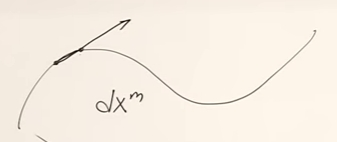
\includegraphics{gr-4-tangent-vector}
\end{figure}

\begin{align*}
	t^m \triangleq& \frac{d x^m}{ds} \text{, we want this to be constant, so}\\
	dt^n + \Gamma \indices{^n_{mr}} t^r dx^m =& 0\\
	\frac{dt^n}{ds}  =& - \Gamma \indices{^n_{mr}} t^r \frac{dx^m}{ds} \\
	=& - \Gamma \indices{^n_{mr}} t^r t^m \text{, or}\\
	\frac{d^2 x^n }{ds^2}=& - \Gamma \indices{^n_{mr}} t^r t^m \text{, equation of motion of a geodesic}
\end{align*}

So, if $s$ is increasing with time, the left hand side looks like acceleration, and the equation itself looks like Newton's 2nd law. The right hand side depends on the geometry, and the particles moves in the straightest line possible.

So far we have discussed 3 dimensional space, as Riemann knew it. We now move to Minkowskian space-time, with proper time--Figure \ref{fig:gr-4-minkowski-space}

\begin{figure}[H]
	\begin{center}
		\caption{Distance in Minkowski Space}\label{fig:gr-4-minkowski-space}
		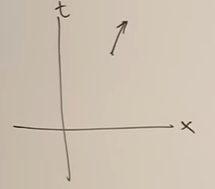
\includegraphics{gr-4-minkowski-space}
	\end{center}
\end{figure}


\begin{align*}
	d \tau^2 =& dt^2 -dx^2 -dy^2 -dz^2\\
	=& - g_{\mu\nu}(x) dx^\mu dx^\nu \text{, where }\\
	g_{\mu\nu} =& \begin{pmatrix}
		-1 &0&0&0\\
		0&1&0&0\\
		0&0&1&0\\
		0&0&0&1
	\end{pmatrix} \numberthis \label{eq:minkowski:metric}\\
	\triangleq& \eta_{\mu\nu} \text{, whence}\\
	d \tau^2=& \eta_{\mu\nu} dx^\mu dx^\nu
\end{align*}

\subsection{Minkowski space}

In 4 dimensions, "flat" means that there is a coordinate system where the metric looks like (\ref{eq:minkowski:metric}).

We want to define a uniformly accelerated motion, but there are problems. \begin{itemize}
	\item If you have a bunch of points which are uniformly separated, \ref{fig:gr-4-uniform-acceleration}, they will maintain a uniform distance, but distances are supposed to transform when they accelerate. If we did this, we'd find the distances getting larger in the rest frame, stretching the strings joining the points, eventually breaking them.
	\item Also the points eventually move faster than the speed of light.
\end{itemize}

\begin{figure}[H]
	\caption{There is a problem defining uniform acceleration in Special Relativity }\label{fig:gr-4-uniform-acceleration}
	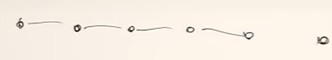
\includegraphics{gr-4-uniform-acceleration}
\end{figure}

We will use an analogue of polar coordinates.

\begin{figure}[H]
	\caption{Constant Acceleration}
	\begin{subfigure}[t]{0.45\textwidth}
		\caption{If the point moves with uniform angular velocity on the circle, the acceleration is uniform, and directed toward the centre.}\label{fig:gr-4-polar}
		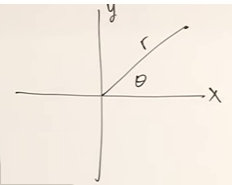
\includegraphics[width=\textwidth]{gr-4-polar}
	\end{subfigure}
	\begin{subfigure}[t]{0.45\textwidth}
		\caption{Constant acceleration in Special Relativity}\label{fig:gr-4-polar-sinh}
		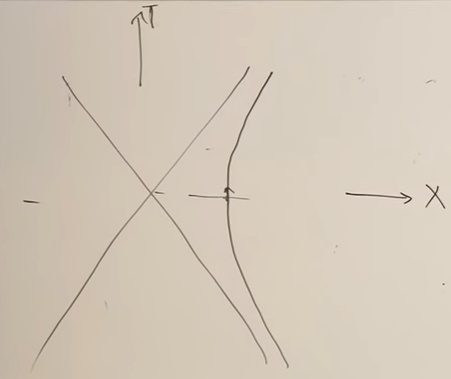
\includegraphics[width=\textwidth]{gr-4-polar-sinh}
	\end{subfigure}
\end{figure}

In Figure \ref{fig:gr-4-polar}
\begin{align*}
	x=& r \cos \theta\\
	y=& r \sin \theta\\
	\cos^2 \theta + \sin^2 \theta =& 1\\
	x^2 + y^2 =& r^2\\
	\cos \theta =& \frac{e^{i \theta}+e^{-i \theta}}{2}\\
	\sin \theta =& \frac{e^{i \theta}-e^{-i \theta}}{2i}
\end{align*}

If the point moves with uniform angular velocity on the circle, the acceleration is uniform, and directed toward the centre.

Figure \ref{fig:gr-4-polar-sinh} depicts constant acceleration in Special Relativity. We replace the trigonometric function by hyperbolic cosines and signs, and the angle $\theta$ is replaces by $\omega$, which increases uniformly. The $\omega$ is like time.

\begin{align*}
	\cosh \omega =& \frac{e^\omega+e^{-\omega}}{2}\\
	\sinh \omega =& \frac{e^\omega-e^{-\omega}}{2}\\
	\cosh^2 \omega +\sinh^2 \omega=& 1\\
	x=& r \cosh \omega\\
	t=& r \sinh \omega\\
	x^2 - t^1 =& 1
\end{align*}

In special relativity $r$ and $\omega$ are the closest thing we have to uniform acceleration--Figure \ref{fig:gr-4-uniform-sinh}. The points along $t=0$ remain the same distance apart as they sweep out their respective hyperbolae.

\begin{figure}[H]
	\begin{center}
		\caption{The closest thing we have to uniform acceleration in special relativity.}\label{fig:gr-4-uniform-sinh}
		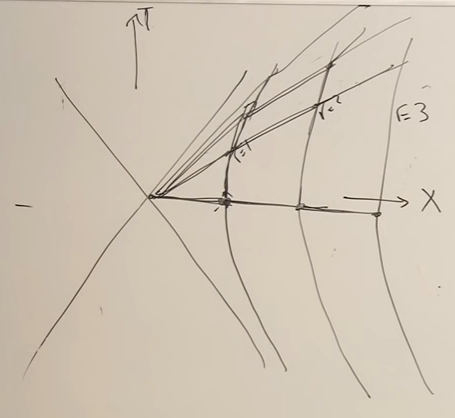
\includegraphics[width=0.8\textwidth]{gr-4-uniform-sinh}
	\end{center}
\end{figure}

Note that the 3 acceleration isn't uniform.

Set:
\begin{align*}
	X=& R \cosh \omega\\
	T=& R \sinh \omega \text{ then the proper acceleration is}\\
	A =& \frac{c^2}{R} \text{, but $c=1$.}
\end{align*}

In hyperbolic polar coordinates
\begin{align*}
	d\tau^2 =& r^2 d \omega^2 - dr^2
\end{align*}

Figure \ref{fig:gr-4-constant-acceleration} depicts constant acceleration.
\begin{figure}[H]
	\begin{center}
		\caption{Constant Acceleration. We go out to a distance R, so acceleration is $g$, then a little further.}\label{fig:gr-4-constant-acceleration}
		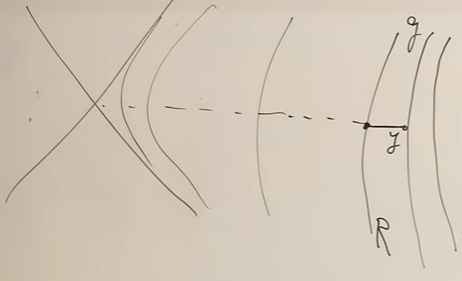
\includegraphics[width=0.8\textwidth]{gr-4-constant-acceleration}
	\end{center}
\end{figure}

At $r=R+y$, the metric is:
\begin{align*}
	d\tau^2 =& \big(R^2 + 2 R y + y^2\big) d \omega^2 - dr^2\\
	=& \big[1 + \frac{2  y}{R} + \big(\frac{y}{R}\big)^2\big] R^2 d \omega^2 - dr^2\\
	=& \big[1 + \frac{2  y}{R} + \big(\frac{y}{R}\big)^2\big] dt^2 - dr^2 \text{, where we define $dt\triangleq R d \omega$}\\
	\approxeq & \big[1 + \frac{2  y}{R} \big] dt^2 - dr^2 \text{, since $y \ll R$}
\end{align*}

The correction accounts for the gravitational force. We'll see this from the equation of motion.

\url{https://youtu.be/YdnLcYNdTzE?list=PLpGHT1n4-mAvcXwzOIz3dHnGZaQP1LEib&t=4624}


\section{Metric for a gravitational field}

TBP

\section{Black holes}

TBP

\section{Falling into a black hole}

TBP

\section{Formation of a black hole}

TBP

\section{Einstein field equations}

TBP

\section{Gravity Waves}

TBP

\bibliographystyle{unsrt}
\addcontentsline{toc}{section}{Bibliography}
\raggedright
\bibliography{tm}

\end{document}
